\section{Dynamic Behavior and Control}

Tilting Narrow Track Vehicles (NTVs) with a high center of mass (CoM) are inherently unstable, necessitating active stabilization to remain upright and controllable. Due to time constraints, a full dynamic controller is beyond the scope of this work. Instead, we demonstrate the viability of steady-state stabilization using a tuned PID controller to maintain balance during straight-line travel and constant-radius turns. The primary goal is to compare the dynamic response of multiple design variants, specifically 3-wheel versus 4-wheel layouts, and rotational versus linear tilt arm mechanisms, under two representative conditions. This results in a total of 8 simulated scenarios. Each simulation is treated as a steady-state configuration, with basic PID control used to stabilize the lean angle. While this does not capture transient or disturbance responses, it is sufficient to evaluate geometry-dependent trends and identify promising configurations for further development.


\subsection{Methodology}

The simulation framework was built using PyBullet, a real-time physics engine. Each vehicle configuration was modeled using a URDF file that specifies link geometry, mass distribution, and joint constraints. Four base configurations were created by combining two platform layouts (three-wheel and four-wheel) with two leaning mechanisms (pivot-based and linear-guided). Each of these was simulated under two scenarios: straight-line motion and constant-radius turning, yielding eight unique scenarios. The straight line scenario occurred on a bumpy surface, while the Curved scenario operated on a flat surface.

For each configuration, the lean angle was controlled via a custom PID controller implemented in the simulation loop. The system was initialized at rest and brought to a constant velocity. For turning scenarios, a fixed-radius turn was imposed by constraining the trajectory. The controller was responsible for adjusting the lean angle to balance centrifugal forces during turning or gravitational instability during straight-line motion.

All simulations recorded joint states (position, velocity, acceleration) and key global metrics such as vehicle lean angle, lateral deviation, and applied control torque. Screenshots of each configuration were captured to document visual differences and posture under dynamic conditions.

\subsection{Implementation}

Each vehicle model is defined using a modular URDF structure, with separate subtrees for chassis, suspension, and lean mechanism. The joint-level PID controller operates within the PyBullet simulation loop at a frequency of 240 Hz. The control law follows:

\[
\tau = K_p(\theta_{\text{desired}} - \theta) + K_d(\dot{\theta}_{\text{desired}} - \dot{\theta}) + K_i \int (\theta_{\text{desired}} - \theta) \, dt
\]

where $\tau$ is the control torque, $\theta$ is the lean joint state, and $\dot{\theta}$ is its velocity. Gains $K_p$, $K_i$, and $K_d$ were manually tuned for each configuration to achieve stable convergence and minimize oscillation.

Data was logged for plotting and post-processing. Camera control was implemented to enable 3D inspection of vehicle motion and stability during runtime, facilitating visual validation of lean behavior and dynamic posture. The figure \ref{fig:actuator-configs} show how the different configuration were implemented in pybullet. The Base mass was set to 100 [kg] while the wheel and segment mass were set to 1 [kg] to emphasize the high CoM.

\newpage

\begin{figure}[h!]
    \centering
    \begin{subfigure}[b]{0.45\linewidth}
        \centering
        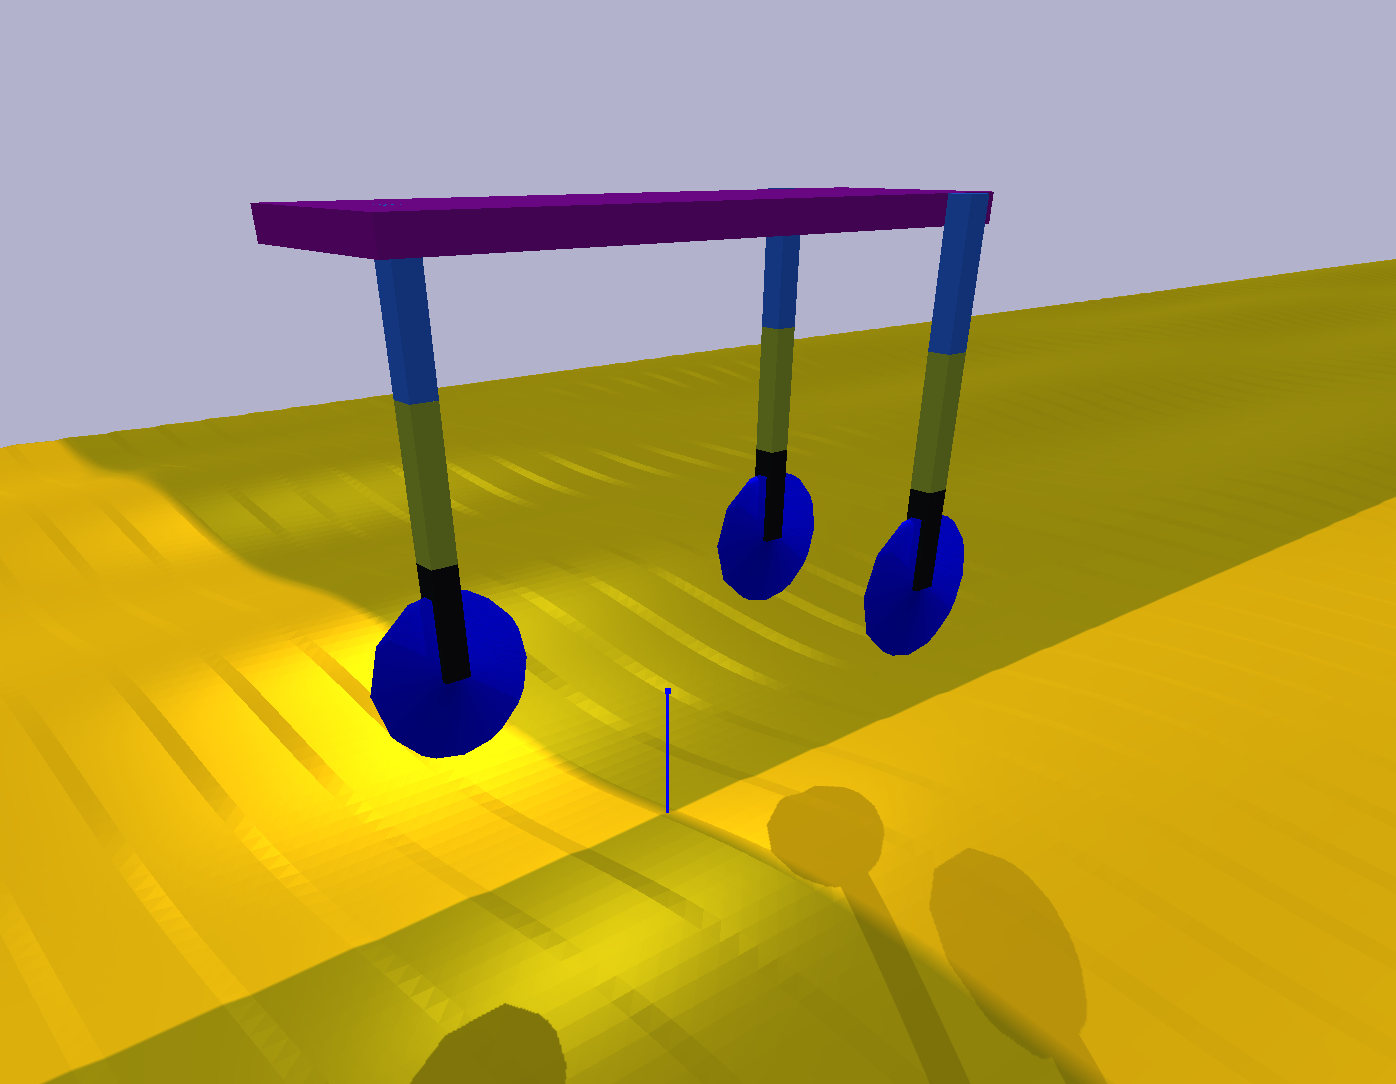
\includegraphics[width=\linewidth]{Figures/ch8_LinearThreeWheel.png}
        \caption{Three Wheeler With Linear Actuator}
    \end{subfigure}
    \hfill
    \begin{subfigure}[b]{0.45\linewidth}
        \centering
        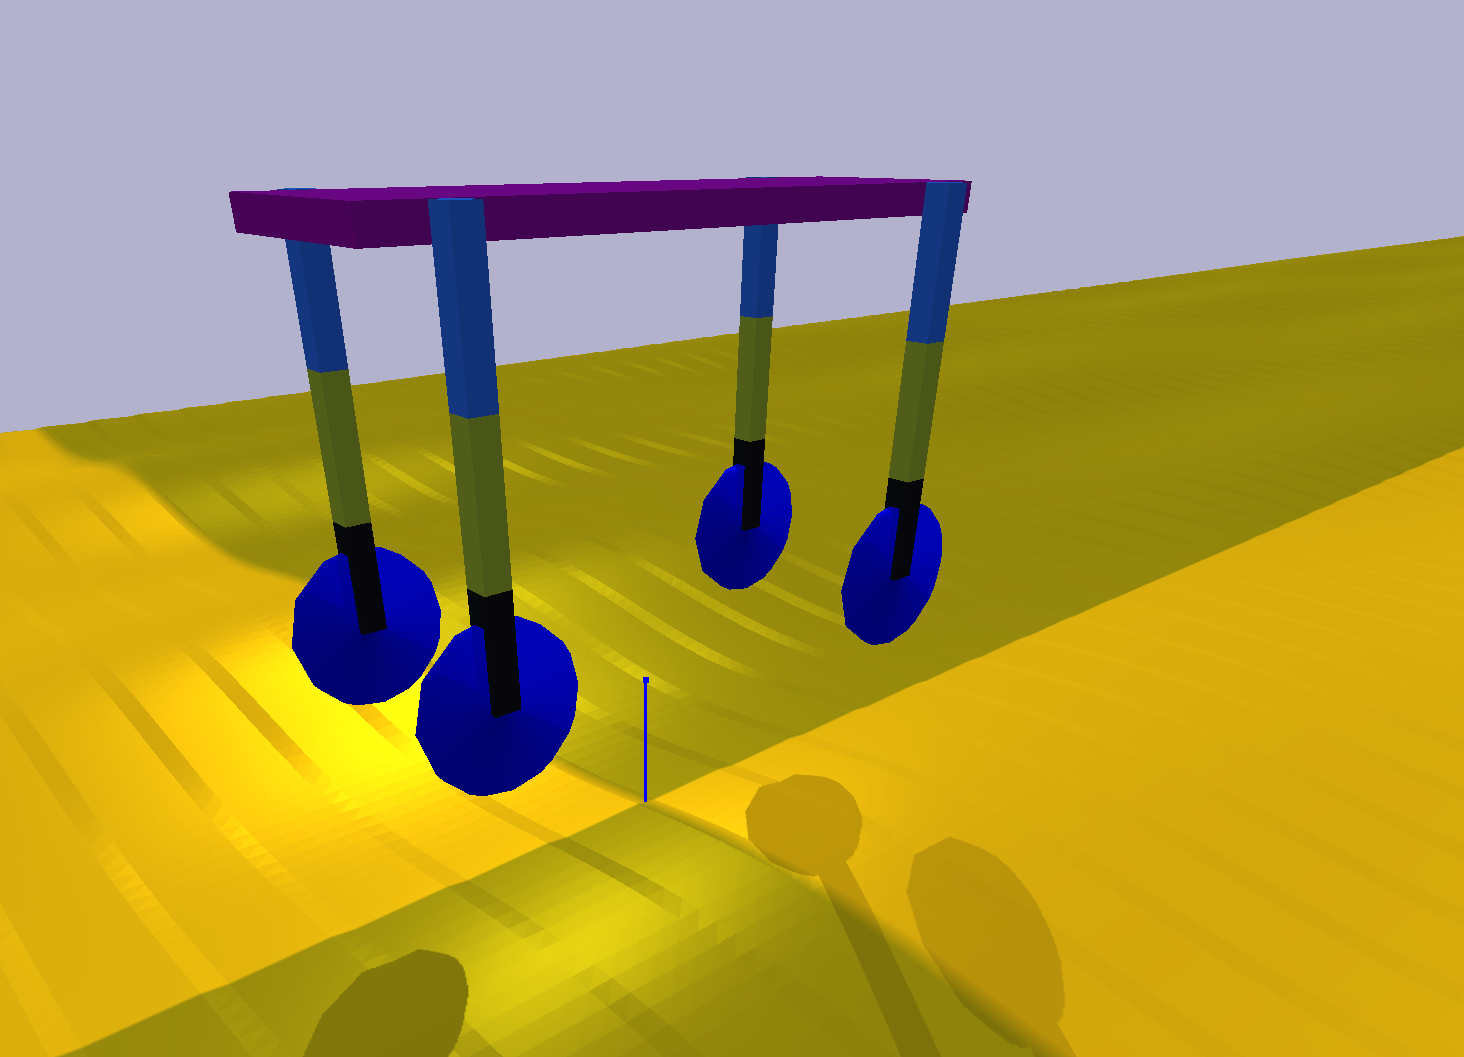
\includegraphics[width=\linewidth]{Figures/ch8_LinearFourWheel.png}
        \caption{Four Wheeler With Linear Actuator}
    \end{subfigure}
    
    \vspace{0.5cm}
    
    \begin{subfigure}[b]{0.45\linewidth}
        \centering
        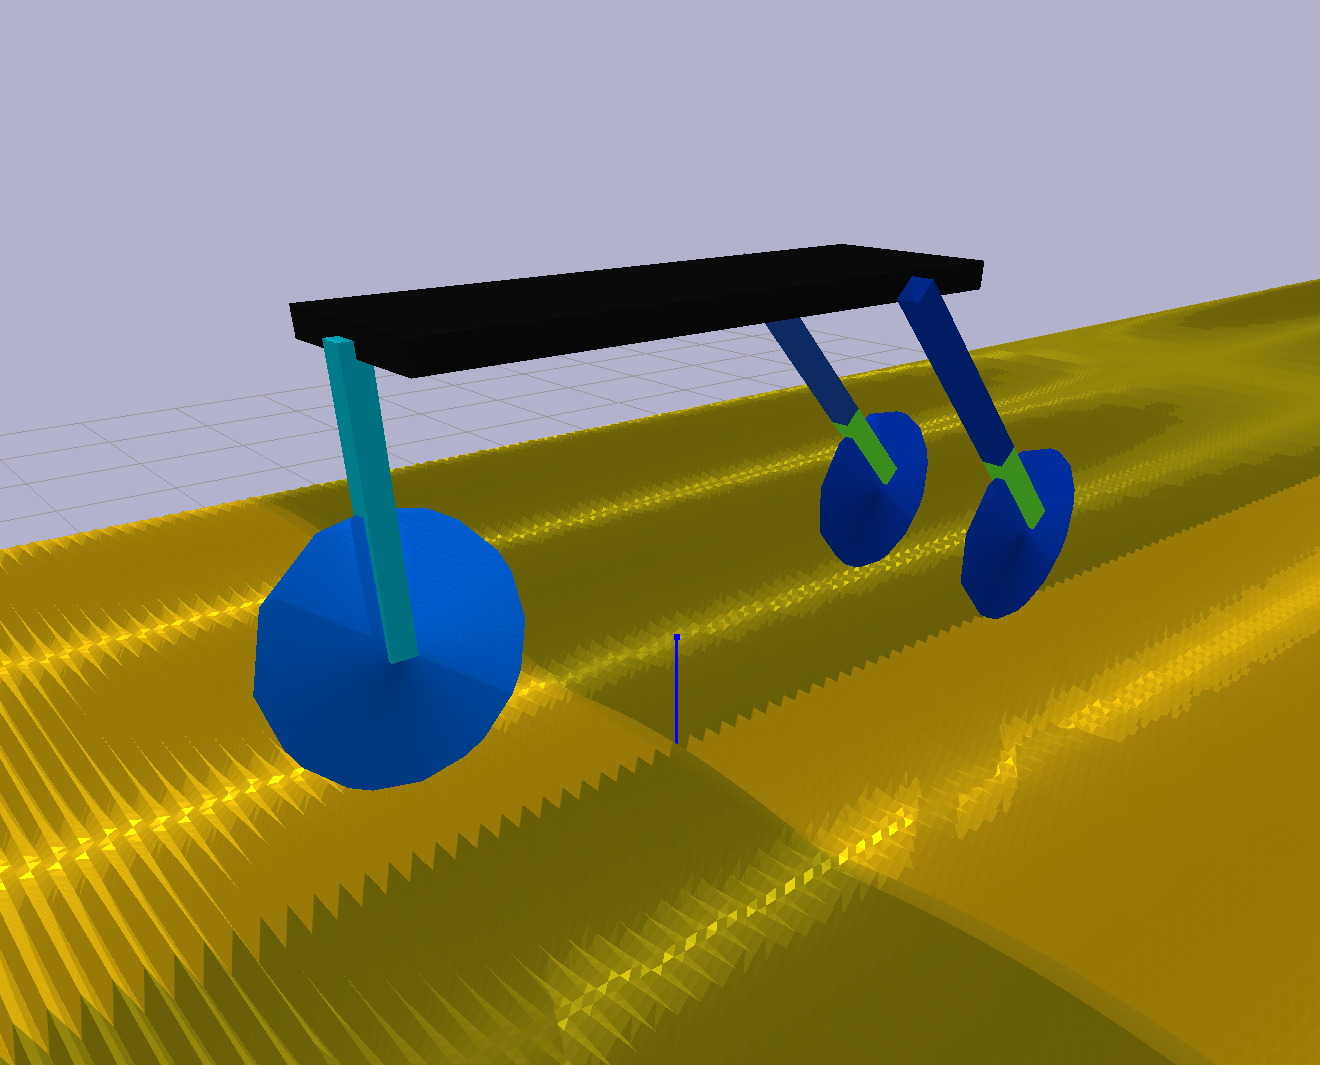
\includegraphics[width=\linewidth]{Figures/ch8_PivotThreeWheel.png}
        \caption{Three Wheeler With Pivot Actuator}
    \end{subfigure}
    \hfill
    \begin{subfigure}[b]{0.45\linewidth}
        \centering
        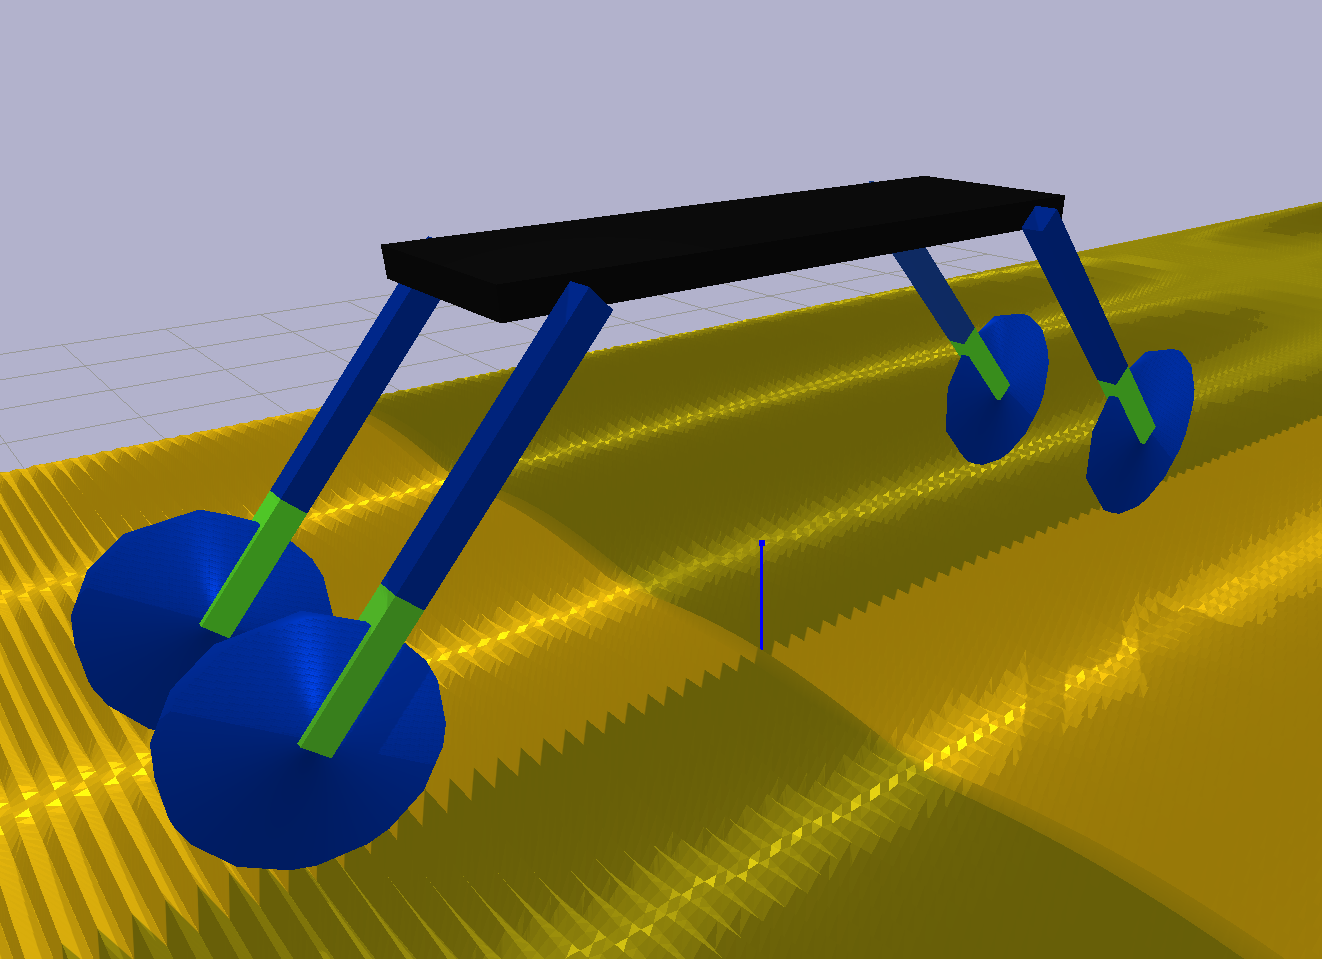
\includegraphics[width=\linewidth]{Figures/ch8_PivotFourWheel.png}
        \caption{Four Wheeler With Pivot Actuator}
    \end{subfigure}
    
    \caption{Comparison of Linear and Pivot Actuated Configurations for Three- and Four-Wheel Designs}
    \label{fig:actuator-configs}
\end{figure}

\subsection{Results}


Qualitatively, I observed for the Pivot design family that the mechanical trail of the wheel (the wheel is further behind the pivot) inscrease stability

Wheel osccilation appear as speed increase. increasing damping solve the problem but might make the response sluggish once we consider the dynamic behaviour.

Pivot arm seems to be fundamentally a flawed idea. The mass of the system push on the wheel and will make them tend to either go inward or outward...

\begin{figure}[h!]
    \centering
    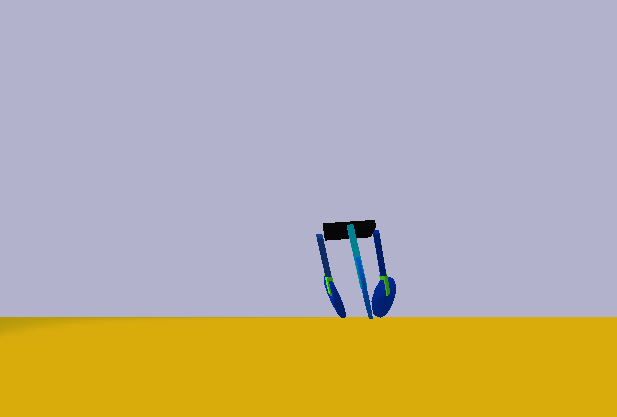
\includegraphics[width=0.5\linewidth]{Figures/ch7_inwardWheel.png}
    \caption{wheel instability on Pivot based Design}
    \label{fig:wheel_instability}
\end{figure}

\begin{figure}
    \centering
    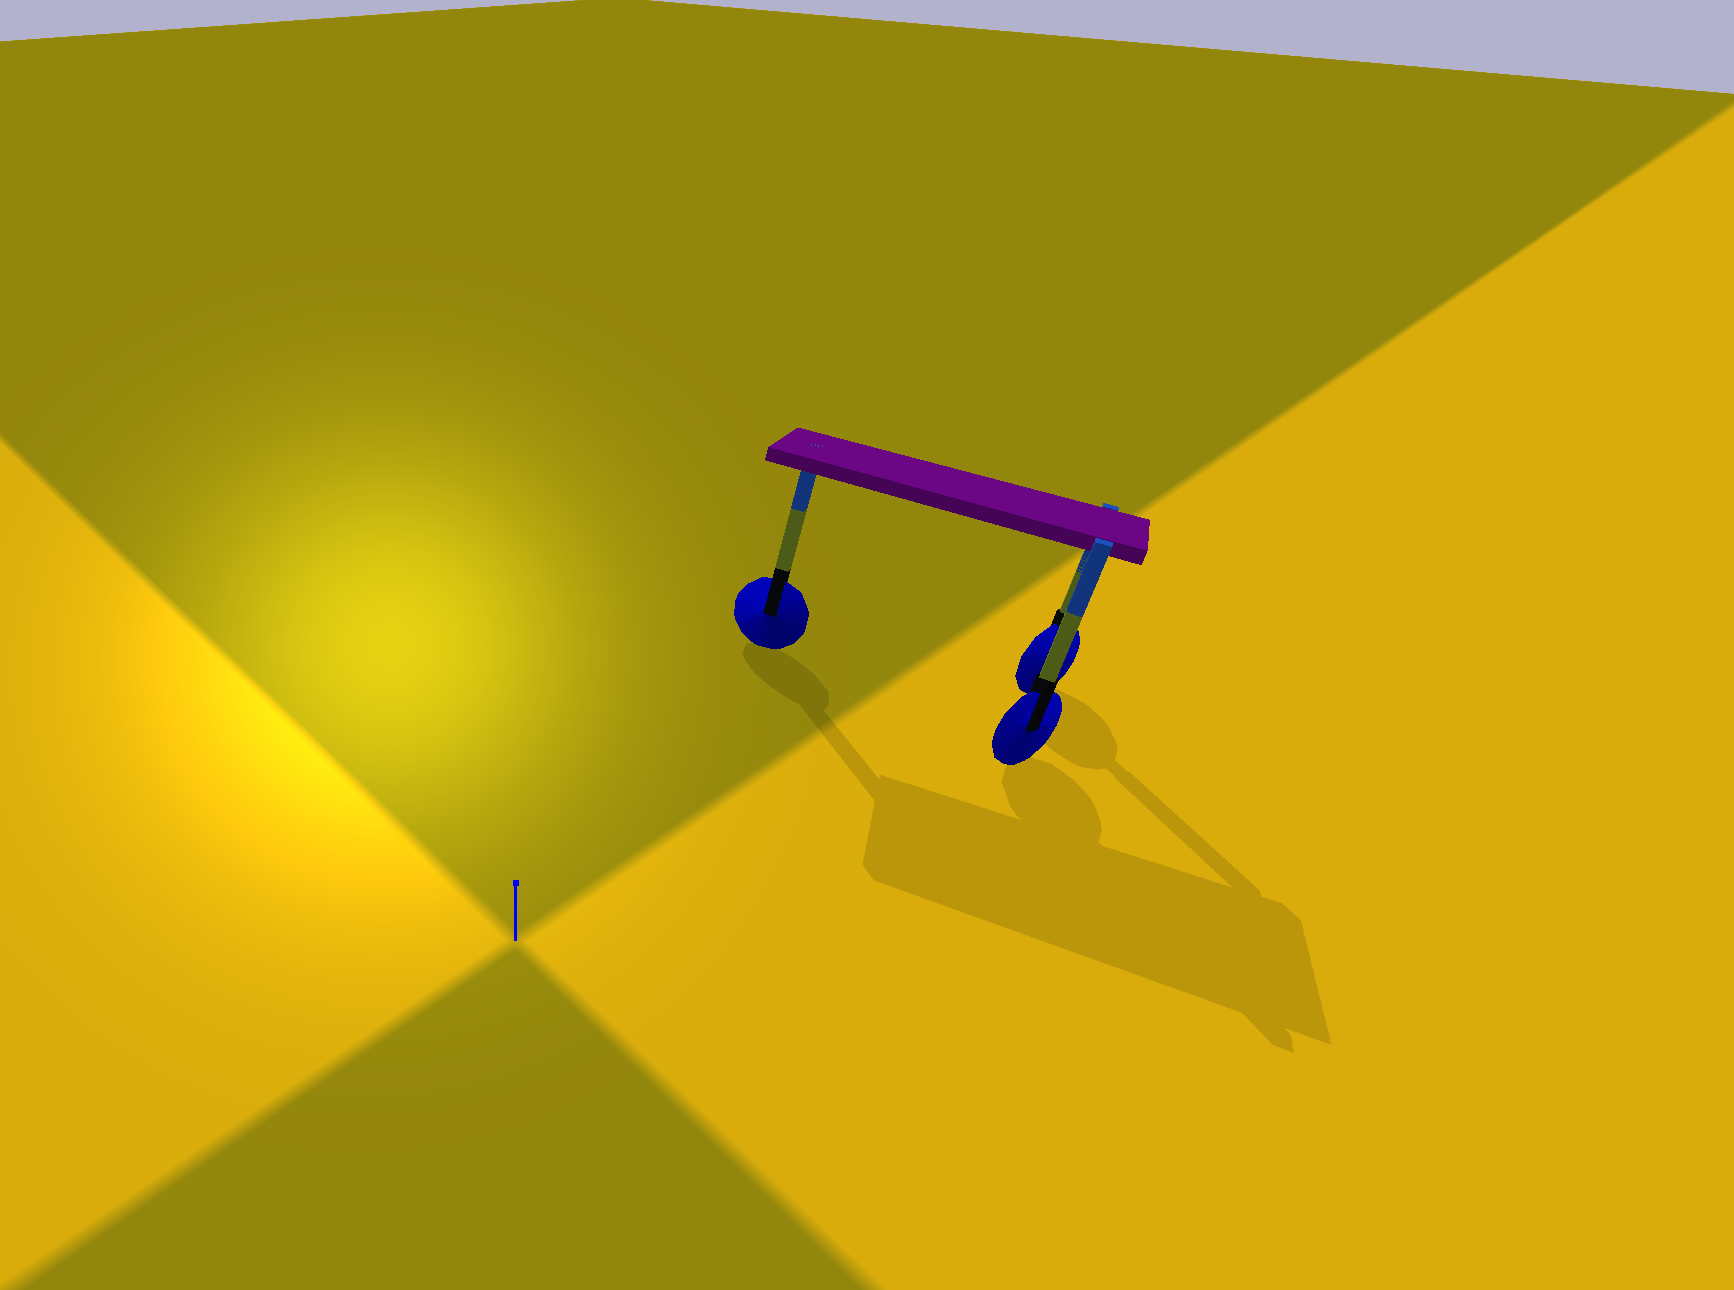
\includegraphics[width=0.5\linewidth]{Figures/ch8_ThreeWheelLinearTurning.png}
    \caption{Sucessful steady state turn for Linear axis based Design}
    \label{fig:linear_success_turn}
\end{figure}